\begin{figure}
  \centering 
  {\fontfamily{pag}\selectfont  
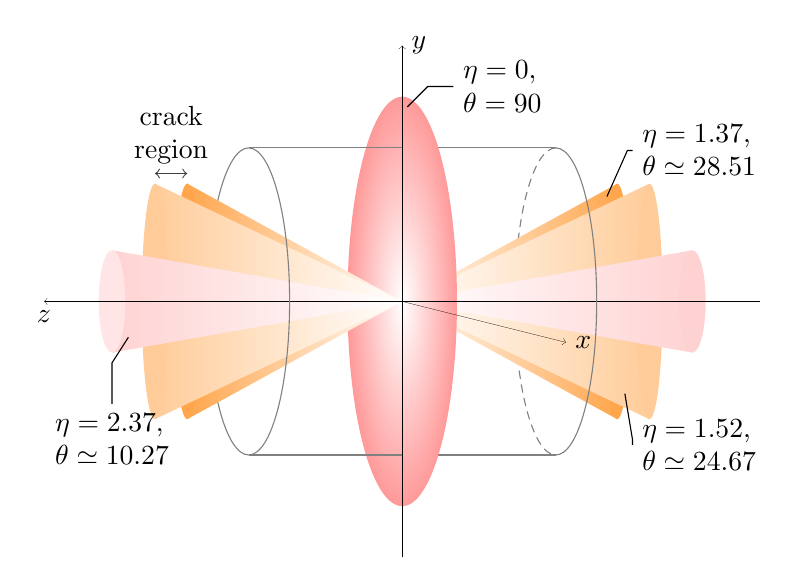
\begin{tikzpicture}[scale=0.65]
	\draw[gray,densely dashed] (3,3) arc[x radius = 0.8, y radius = 3, start angle= 90, end angle= 270];
	\draw[gray] (-3,3) arc[x radius = 0.8, y radius = 3, start angle= 90, end angle= 270];
	\draw[gray] (3,3) -- (0,3); \draw[gray] (3,-3) -- (0,-3);
	
	%eta1.37
	\draw[right color=orange!70!white, left color=white,draw=none] (0,0)--(4.2,2.3)--(4.2,-2.3) --cycle;
	\draw[fill=orange!70!white,draw=none] (4.2,2.3)arc[x radius = 0.26, y radius = 2.3, start angle= 90, end angle= 450];
	\draw[thin] (4,2.05) -- (4.4,2.95) -- (4.5,2.95) node[right,align=left] {$\eta=1.37$, \\$ \theta\simeq\ang{28.51}$};

	%eta1.52
	\draw[right color=orange!40!white, left color=white,draw=none] (0,0)--(4.83,2.3)--(4.83,-2.3) --cycle;
	\draw[fill=orange!40!white,draw=none] (4.83,2.3)arc[x radius = 0.26, y radius = 2.3, start angle= 90, end angle= 450];
	\draw[thin] (4.35,-1.8) -- (4.5,-2.7) -- (4.5,-2.8) node[right,align=left] {$\eta=1.52$, \\$ \theta\simeq\ang{24.67}$};
	
	%eta2.37
	\draw[right color=pink!70!white, left color=white,draw=none] (0,0)--(5.67,1)--(5.67,-1) --cycle;
	\draw[fill=pink!70!white,draw=none] (5.67,1)arc[x radius = 0.26, y radius = 1, start angle= 90, end angle= 450];

	
	%eta0
	\draw[inner color =white, outer color=red!40!white,draw=none] (0,0) ellipse (1.07 and 4);	
	\draw[thin] (0.1,3.8) -- (0.5,4.2) -- (1,4.2) node[right,align=left] {$\eta=0,$ \\$ \theta=\ang{90}$};
	
	%eta1.37left
	\draw[left color=orange!70!white, right color=white,draw=none] (0,0)--(-4.2,2.3)--(-4.2,-2.3) --cycle;
	\draw[fill=orange!70!white,draw=none] (-4.2,2.3)arc[x radius = 0.26, y radius = 2.3, start angle= 90, end angle= 450];
	
	%eta1.52left
	\draw[left color=orange!40!white, right color=white,draw=none] (0,0)--(-4.83,2.3)--(-4.83,-2.3) --cycle;
	\draw[fill=orange!40!white,draw=none] (-4.83,2.3)arc[x radius = 0.26, y radius = 2.3, start angle= 90, end angle= 450];
	
	%eta2.37left
	\draw[left color=pink!70!white, right color=white,draw=none] (0,0)--(-5.67,1)--(-5.67,-1) --cycle;
	\draw[fill=pink!40!white,draw=none] (-5.67,1)arc[x radius = 0.26, y radius = 1, start angle= 90, end angle= 450];
	\draw[thin] (-5.35,-0.7)--(-5.67,-1.2) -- (-5.67,-2) node[below,align=left] {$\eta=2.37$, \\$ \theta\simeq\ang{10.27}$};
	
	\draw[<->,darkgray] (-4.83,2.5)--(-4.2,2.5);
	\draw[] node at (-4.515,2.5) [above,align=center]{crack\\ region};
	%\draw[] node at (7.3,-0.3) [right,align=right]{$\eta=\infty,$\\ $\theta=\ang{0}$};

  	\draw [->,ultra thin] (7,0)--(-7,0) node[below]{$z$};
	\draw [->,ultra thin] (0,0)--(3.2,-0.8) node[right]{$x$};
	\draw [->,ultra thin] (0,-5)--(0,5) node[right]{$y$};
	\draw[gray] (-3,3) arc[x radius = 0.8, y radius = 3, start angle= 90, end angle= -90];
	\draw[gray] (0,3) -- (-3,3); \draw[gray] (0,-3) -- (-3,-3);
	
	\draw[gray] (3,-3) arc[x radius = 0.8, y radius = 3, start angle= -90, end angle= 90];

\end{tikzpicture}
}
\caption{Notable value of $\eta$ for the corresponding $\theta$. The crack region  for\etaRange{1.37}{1.52}, along with the limit of photon acceptance in this analysis for $\eta = 2.37$  are highlighted. The cilinder is a sketch of the ATLAS detector. Due to left-right simmetry, the $\theta$ angle displayed represents both the value shown and their $\pi-\theta$ symmetric. When $\theta$ approaches \SI{0}{°}, $\eta$ assumes larger values. \\
All the points on the cone displayed share the same value of pseudorapidity.}
\label{fig:pseudorapidita}
 \end{figure}